%%%%%%%% ICML 2018 EXAMPLE LATEX SUBMISSION FILE %%%%%%%%%%%%%%%%%

\documentclass{article}

% Recommended, but optional, packages for figures and better typesetting:
\usepackage{microtype}
\usepackage{graphicx}
\usepackage{subfigure}
\usepackage{booktabs} % for professional tables
\usepackage{amsmath, amssymb}

\usepackage[utf8]{inputenc}
\usepackage[T1]{fontenc}
\usepackage{hyperref}
\usepackage{url}
\usepackage{booktabs}
\usepackage{amsfonts}
\usepackage{nicefrac}
\usepackage{microtype}
\usepackage{xcolor}
\usepackage{lipsum}
% \usepackage[nomarkers,nolists,figuresonly]{endfloat} %comment out when finish
\usepackage{booktabs}
\usepackage{multirow}
\usepackage{float}
\usepackage{subcaption}


% hyperref makes hyperlinks in the resulting PDF.
% If your build breaks (sometimes temporarily if a hyperlink spans a page)
% please comment out the following usepackage line and replace
% \usepackage{icml2018} with \usepackage[nohyperref]{icml2018} above.
\usepackage{hyperref}

% Attempt to make hyperref and algorithmic work together better:
\newcommand{\theHalgorithm}{\arabic{algorithm}}

% Use the following line for the initial blind version submitted for review:
\usepackage[accepted]{icml2018}

% If accepted, instead use the following line for the camera-ready submission:
%\usepackage[accepted]{icml2018}

% The \icmltitle you define below is probably too long as a header.
% Therefore, a short form for the running title is supplied here:
\icmltitlerunning{CS234: Reinforcement Learning Winter 2025 - Final Project}

\begin{document}

%%%%%%%%%%%%%%%%%%%%%%%%%%%%%%%%%%%%%%%%%%%%%%%%%%%%%%%%%%%%%%%%
%%%%%%%%%%%          HEADER SECTIONS HERE            %%%%%%%%%%%
%%%%%%%%%%%%%%%%%%%%%%%%%%%%%%%%%%%%%%%%%%%%%%%%%%%%%%%%%%%%%%%%


\twocolumn[
\icmltitle{Enhancing Game Control Through \\
Hybrid Reinforcement Learning
}

\begin{icmlauthorlist}
\icmlauthor{Danhua Yan}{to}
\end{icmlauthorlist}

\icmlaffiliation{to}{Department of Computer Science, Stanford University}
\icmlcorrespondingauthor{Danhua Yan}{dhyan@stanford.edu}

% You may provide any keywords that you
% find helpful for describing your paper; these are used to populate
% the "keywords" metadata in the PDF but will not be shown in the document
% \icmlkeywords{Machine Learning, ICML}

\vskip 0.3in
]

% this must go after the closing bracket ] following \twocolumn[ ...

% This command actually creates the footnote in the first column
% listing the affiliations and the copyright notice.
% The command takes one argument, which is text to display at the start of the footnote.
% The \icmlEqualContribution command is standard text for equal contribution.
% Remove it (just {}) if you do not need this facility.

%\printAffiliationsAndNotice{}  % leave blank if no need to mention equal contribution
% \printAffiliationsAndNotice{\icmlEqualContribution} % otherwise use the standard text.
\printAffiliationsAndNotice{} % otherwise use the standard text.



%%%%%%%%%%%%%%%%%%%%%%%%%%%%%%%%%%%%%%%%%%%%%%%%%%%%%%%%%%%%%%%%
%%%%%%%%%%%           MAIN SECTIONS HERE             %%%%%%%%%%%
%%%%%%%%%%%%%%%%%%%%%%%%%%%%%%%%%%%%%%%%%%%%%%%%%%%%%%%%%%%%%%%%


\begin{abstract}
      This document provides a basic paper template and submission guidelines.
      Abstracts must be a single paragraph, ideally between 4--6 sentences long.
      Gross violations will trigger corrections at the camera-ready phase.
      This document provides a basic paper template and submission guidelines.
      Abstracts must be a single paragraph, ideally between 4--6 sentences long.
      Gross violations will trigger corrections at the camera-ready phase.
      This document provides a basic paper template and submission guidelines.
      Abstracts must be a single paragraph, ideally between 4--6 sentences long.
      Gross violations will trigger corrections at the camera-ready phase.
      This document provides a basic paper template and submission guidelines.
      Abstracts must be a single paragraph, ideally between 4--6 sentences long.
      Gross violations will trigger corrections at the camera-ready phase.
      This document provides a basic paper template and submission guidelines.
      Abstracts must be a single paragraph, ideally between 4--6 sentences long.
      150 words.
\end{abstract}

\section{Introduction}

% What is the problem that you will be investigating ? Why is it interesting ?
% What literature have you already surveyed or will be 
% examining to provide context and background ?

Training reinforcement learning (RL) agents typically demands substantial 
data and exploration to achieve optimal performance. In complex environments 
such as difficult retro arcade games, high-dimensional state spaces, sparse rewards, 
and intricate dynamics make pure exploration particularly inefficient. 
Moreover, situations with limited or costly exploration opportunities 
increase the risk of converging to suboptimal policies.

To address these challenges, hybrid RL (HRL) paradigms leveraging demonstrations 
and imitation learning (offline RL) combined with agent exploration (online 
RL) have emerged as effective solutions. Specifically, Behavior Cloning (BC) 
integrated with Proximal Policy Optimization (PPO) has shown considerable 
potential. These hybrid methods use human demonstrations to bootstrap initial 
policies, significantly accelerating learning, with the potential to converge 
to policies that surpass demonstration performance levels.

This study investigates approaches that integrate human-generated 
demonstrations into PPO training, focusing on techniques such as transfer 
learning from BC, KL divergence-based regularization, and assisted exploration 
strategies in a complex retro game environment.

\section{Related Work}
Behavior cloning (BC) effectively initializes reinforcement learning 
policies using human demonstrations to tackle challenging exploration 
problems. It often trains faster than RL agents, providing a solid 
starting point for explorations.

PPO weight initialization via transfer learning is a common strategy. A BC 
policy network is first trained through supervised learning on human 
demonstration data. These pre-trained weights are then used to 
initialize PPO training. The DQfD approach by \cite{hester_dqfd_2017} 
combines behavior cloning and DQN networks, demonstrating effective 
training and surpassing demonstration performance. 
\cite{laidlaw2024bridgingrltheorypractice} shows BC weights 
initiated PPO using Atari-HEAD human datasets, indicating notable 
efficiency gains, especially for tasks with extended exploration 
phases and sparse rewards. \cite{Coletti2023EffectivenessOW} 
demonstrates that PPO warm-started with expert demonstrations can 
achieve satisfactory results in the costly exploration field of 
controlling a fixed-wing unmanned aerial vehicle. This approach 
significantly reduces the initial exploratory behavior required by 
the agent, leading to substantial improvements in sample efficiency 
and faster convergence.

Another common approach is to integrate behavior cloning into PPO by 
adding a divergence-based regularization term, typically the 
Kullback-Leibler (KL) divergence, between the current PPO policy and 
a reference BC policy. This regularization guides the PPO agent to 
remain close to behaviors suggested by human demonstrations, 
especially early in training. This method is similar to the 
Kickstarting framework by \cite{schmitt2018kickstartingdeepreinforcementlearning}, 
where an auxiliary distillation loss encourages the student policy to 
follow the teacher (reference) policy initially, progressively 
allowing divergence as training advances to surpass human performance.

Assisted exploration leverages demonstrations to guide agent exploration 
explicitly, often through curriculum strategies that reset or start episodes 
from states sampled from human demonstrations. This approach does not require 
a BC network but uses human trajectories to shape the exploration process, 
enhancing learning efficiency and performance.
The idea is to reset the agent 
to progressively more challenging starting points, encouraging the learning 
process \cite{florensa2018reversecurriculumgenerationreinforcement}. 
\cite{salimans2018learningmontezumasrevengesingle} illustrate this in Atari's 
Montezuma’s Revenge, using demonstration states to reduce exploration 
complexity and improve learning outcomes. This form of assisted exploration 
allows the agent to efficiently encounter and practice critical, sparse-reward 
regions of the state space, enhancing PPO's capability to master challenging 
tasks that conventional random exploration methods struggle with.

In this study, we explore the efficacy of HRL paradigms in a retro game 
environment.


\section{Data and Environement}
In this project, we leverage the \texttt{stable-retro} library to create an OpenAI Gym 
environment for training an agent to play the NES game Super Mario Bros, level 1-1. The 
default integration of the environment encapsulates the game into the in-game visual 
frame as a matrix $I \in \mathbb{R}^{H \times W \times 3}$, where each element takes an 
integer value between 0 and 255, representing the RGB channels of the frame. The action 
of pressing 9 buttons on NES controllers is represented as a vector 
$\mathbf{a} = (a_1, a_2, \dots, a_9) \in \{0, 1\}^9$, where each button can be toggled 
independently, resulting in a total of 512 discrete action spaces. The default reward 
is the change in the $x$-axis position $\Delta x$ moved by Mario. In-game metadata, including 
scores, time left, and positions of Mario, can also be retrieved for each timestep $t$.

\subsection{Human Demonstration Data}
\label{sec:hd_data}
To record human demonstrations, we implemented scripts to save gameplay 
interactions with the environment via a game controller. 
We recorded five gameplays by amateur players $\{\tau_{\text{HD}}^{i}\}_{i=1}^{5}$, 
each successfully completing Level 1-1 without losing a life.
Each episode $i$ is 
saved as $\tau_{\text{HD}}^{i} = \{(s_t, a_t, r_t, d_t, m_t)\}_{t=0}^{T}$, where each 
element represents the observation, action, reward, termination boolean, and 
metadata.  
Additionally, a single trajectory 
of game emulator states is saved every 50 steps, 
$\tau_{\text{ES}} = \{ s_t \mid t \in \{ 50k \mid k\in \mathbb{N}, 50k \leq T \} \}$,
used for resetting RL agents 
to start from a state along the human demonstrated trajectory.

\subsection{Customized Game Environement}

To frame the game as a solvable RL problem within a reasonable time, we made 
the following custom modifications to the default game integration:

\textbf{Action Space} 
The default 512 discrete action space includes all possible joystick button 
combinations, most of which are not meaningful for controlling Mario. We 
reduced the action space to 3 commonly used button combinations (see 
Appendix \ref{a1:custom_env}).

\textbf{Termination States}
The default game termination occurs when Mario exhausts all lives or the 400 
second time limit for Level 1-1 is reached. We employ stricter termination 
conditions: 1) Mario has only one life, and the game terminates immediately if 
he loses it; 2) If Mario remains stuck at the same position without moving 
right for 10 seconds, the game is terminated.

\textbf{Reward Function}
\label{sec:reward}
The game's scoring system provides sparse rewards for defeating enemies, 
collecting coins or power-ups, and successfully completing the level.
We modify the reward function to provide dense rewards, incorporating scores, 
encouraging rightward movement with milestones, and penalizing time consumption 
and termination without success:

\begin{align*}
      \mathcal{R} = &\Delta s + \beta_x \Delta x + \beta_t \Delta t + \mathbf{1}[d_{\text{milestones}} = 1] M\\
      & + \mathbf{1}[d_{\text{timeout}} = 1] T_t + \mathbf{1}[d_{\text{death}} = 1] T_d
\end{align*}

where $\Delta s$ is the score earned since the last state, $\Delta x$ is the 
movement, $\Delta t$ is the time spent, $\beta$ are coefficients, $M$ is the 
milestone score at 10\%, 20\%, etc., of the level, and $T_t$ and $T_d$ are 
penalties for timeout and death terminations.

\textbf{Sampling Rate}
To ensure smooth rendering, the game runs at 60 fps. However, consecutive 
frames exhibit minimal differences. Following \cite{feng2024mario}, 
we reduced the sampling rate to 15 fps to reduce state spaces.


\section{Approach}
In this section, we describe baseline and three different hybrid reinforcement 
learning approaches in controlling Mario for completing level 1-1.

\subsection{Policy Training Architectures}

\begin{figure}[htbp]
      \centering
      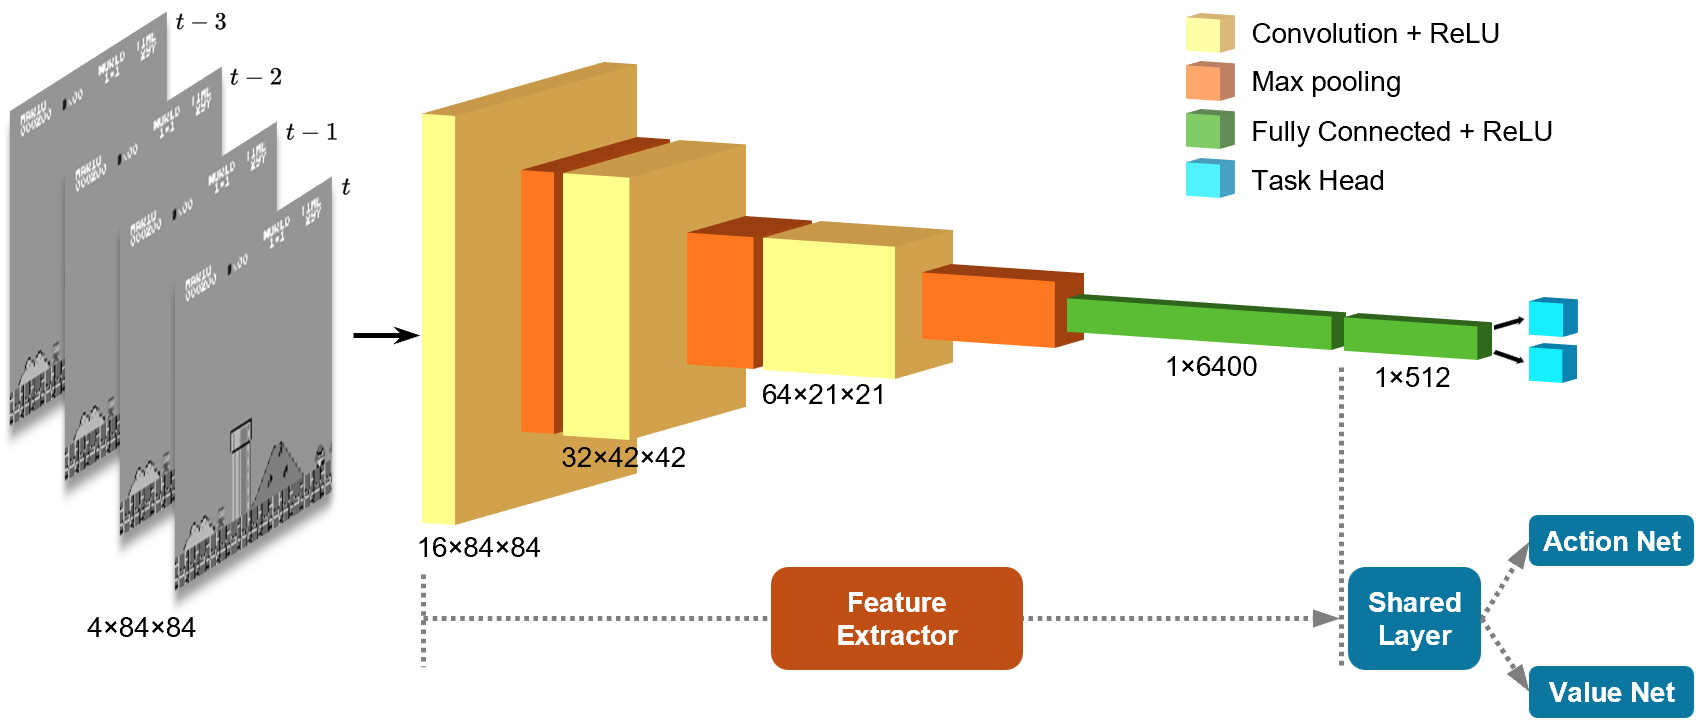
\includegraphics[width=\columnwidth]{figures/architecture.png}
      \caption{PPO agent architecture for playing Super Mario Bros.
      Four downsampled gameplay frames are stacked 
      to represent the current state $s_t$, as input to the CNN actor-critic PPO
      networks.}
      \label{fig:arch}
\end{figure}

\textbf{State Representation}
Due to the presence of moving enemies (\textit{e.g.}, Goombas, Koopa Troopas) 
and power-ups, \textit{Super Mario Bros.} exhibits non-Markovian dynamics.
As a result, incorporating temporal structure in the state representation is 
crucial for accurately estimating enemy movements and other dynamic changes. 
To capture these temporal dependencies, we define the state $s_t$ at time $t$ 
as a stack of four consecutive gameplay frames, $\{ f_{t-3}, \dots, f_t \}$, 
preserving local temporal dynamics (see Figure \ref{fig:arch}). 
Each frame is downsampled from its original RGB representation to a 
single-channel grayscale image and resized to $84 \times 84$ pixels.

\textbf{Network Architectures}
All baselines and HRL approaches use the same architecture 
(Figure \ref{fig:arch}). The feature extractor is a CNN 
$\phi_s = \mathcal{F}(s;\phi)$ that maps the stacked state 
representation \(4 \times 84 \times 84\) to a dense feature 
representation. The CNN has three convolutional layers with 16, 32, 
and 64 channels, respectively. Each convolution uses a \(3 \times 3\) 
kernel with stride 1 and padding 1, followed by ReLU activation and 
\(2 \times 2\) max pooling, halving the spatial dimensions. 
The PPO actor-critic policy 
is a multi-head MLP network $a, V = \mathcal{M}(\phi_s; \theta)$ with a 
shared fully connected hidden layer of 512 units and 
ReLU activation, and two linear heads:
the action net $ \pi_\theta(a|s) = M_a(\phi_s;\theta_a)$,
and the value net ${\hat V}(s) = M_V(\phi_s;\theta_V)$.
For BC, it matches the PPO with just action net:
$ \pi_{\text{BC}}(a|s) =
\mathcal{M}_{\text{BC}}(\mathcal{F}(s;\phi_{\text{BC}});\theta_{\text{BC}})$.


\subsection{Baselines}
Here we shall establish performance of offline-only and online-only RL approaches
as baselines to compare against future HRL approaches and human demonstration trajectories. 

\subsubsection{Behavior Cloning (BC)} 
BC is an offline approach using supervised 
learning to map state-action pairs from human demonstrations. We learned 
a BC policy $\pi_{\text{BC}}(a|s) =
\mathcal{M}_{\text{BC}}(\mathcal{F}(s;\phi_{\text{BC}});\theta_{\text{BC}})$
using $(s,a)$ pairs from human demonstration data $\tau_{\text{HD}}$ as mentioned
in section \ref{sec:hd_data}.

\subsubsection{Proximal Policy Optimization (PPO)} 
PPO serves as an online baseline. We extended the 
\texttt{stable-baseline3} PPO implementation, utilizing the 
CNN feature extractor $\mathcal{F}(s;\phi)$ and the two-head 
MLP policy network $a, V = \mathcal{M}(\phi_s; \theta)$. 
Parameters $\phi$ and $\theta$ are updated via gradient 
descent per rollout iteration.
Here we denote the policy learned by PPO as 
$\pi_\theta(a|s) = M_a(\mathcal{F}(s;\phi);\theta_a)$.


\subsection{Hybrid Reinforcement Learning (HRL)}
We explore three HRL paradigms, leveraging pre-trained BC policies or 
directly using human demonstration data in PPO policy learning.

\subsubsection{BC-Initialized PPO}
This approach initializes PPO explorations using pre-trained behavior 
cloning weights. These weights provide a biased prior for state and 
action distributions, giving the agent a reasonable initial policy 
for exploration. 
Instead of initializing the model with random parameters 
$\phi_0$ and $\theta_0$, i.e., $a, V = \mathcal{M}_0(\mathcal{F}_0(s;\phi_0); 
\theta_0)$, we warm-start the feature extractor $\phi_0 \leftarrow 
\phi_{\text{BC}}$ and/or the policy network $\theta_0 \leftarrow 
\theta_{\text{BC}}$ in this approach.

\subsubsection{BC-Constrained PPO}
This approach constrains the PPO policy to remain close to the pre-trained BC 
policy by adding a KL-divergence term to the loss function:

\begin{align*}
      \mathcal{L}(\theta) 
      &= \mathcal{L}_{\text{PPO}}(\theta) +
      \lambda \mathbb{E}_{s \sim \mathcal{D}} \bigg[ \sum_{a} \pi_{\theta}(a | s) \log 
      \frac{\pi_{\theta}(a | s)}{\pi_{\text{BC}}(a | s)} \bigg],
\end{align*}
where $\mathcal{L}_{\text{PPO}}$ is the default PPO loss, $\lambda$ is the hyperparameter
controlling the strength of the divergence loss.

\subsubsection{Assisted Explorations}
This approach aims to shape the exploration process using human trajectories. 
The key idea is to reset the rollout to progressively more challenging starting 
points for the agent, encouraging the learning process \cite{florensa2018reversecurriculumgenerationreinforcement}. 
\cite{salimans2018learningmontezumasrevengesingle} proposed reversing the human 
gameplay trajectory as resets to effectively encourage learning. Inspired by 
their approach, we propose a simpler version of resets using an exponential 
decay schedule, instead of running indefinitely until each reset reaches a 
certain performance threshold.

The exponential decay schedule for PPO resets works as follows: given a target 
training iteration count $N$ and $k$ resets along the trajectory, we want the 
$i$-th state to be reset for rollout $f(i)$ times, such that $f(i)$ follows a 
discrete exponential distribution $f(i) \sim r^i$, and $\sum_{i=1}^{k} f(i) 
\approx N$. Here, $r$ is the decay factor, where $0 < r < 1$, that smaller $r$ decays 
faster. The PPO rollouts start from the $k$-th human state from 
$\tau_{\text{ES}}$ (see section \ref{sec:hd_data}) $f(k)$ times, then move to 
the $(k-1)$-th state $f(k-1)$ times, and so on, until exhausting all states in 
$\tau_{\text{ES}}$. If there are still training steps remaining, the rollouts 
start from the initial state $s_0$.

The intuition behind this approach is to distribute resets strategically 
within a given training iteration count. States closer to the winning 
state (later states) are easier and thus get less practice than the 
earlier, more difficult states. This schedule effectively distributes 
learning along good state trajectories within limited training time, 
aiding efficient explorations.




\section{Experiments}
In this section, we present experimental results for the aforementioned 
approaches. 

\subsection{Experimental Details}
All experiments are trained on a single Nvidia GeForce RTX 4070 Ti 
SUPER 16GB GPU. Random seed is set to 12345 for consistency.

\textbf{Reward Function} We set coefficients of reward function described
in section \ref{sec:reward} as time coefficient $\beta_t = -1$, 
position coefficient $\beta_x = 0.1$, 
$M=1000m$, where $m=\{0.1, 0.2, \cdots, 1\}$ is the game completion percentage.
Timeout termination $T_t = -1000$, death termination $T_d = -1000$.

\textbf{Behavior Cloning} All $(s_t, a_t)$ 
pairs from human demonstration $\tau_{\text{HD}}$ are split into \texttt{train} and \texttt{dev} sets in a 7:3 ratio. 
With a batch size of 32 and cross-entropy loss, the full network 
$\pi(\mathcal{F}(s; \phi);\theta)$ is trained for 500 epochs using 
AdamW optimizer with a learning rate of $10^{-4}$. Early termination 
occurs after 50 epochs based on \texttt{dev} data accuracy.

\textbf{PPO and HRL Extensions} In each iteration, the agent rolls out for 
512 steps and updates the networks for 10 epochs with a batch size of 32, 
over 200 iterations. We set an entropy loss coefficient of 0.01. For 
BC-constrained PPO, $\lambda=0.1$ for KL-divergence loss regularization. For 
baseline PPO, BC-constrained PPO, and assisted exploration methods, we use 
a learning rate of $10^{-4}$, a clip range of $0.1$. For BC-initialized 
PPO, we use a smaller learning rate of $1\times10^{-5}$ and a linear clip 
range schedule starting from 0.05 to 0.15. This stabilizes PPO near the BC 
policy initially and later encourages policy updates to potentially surpass 
demonstration strategies. For assisted explorations, we have $k=43$ resets 
along demonstration $\tau_{\text{ES}}$, with $r=0.9$ and $N=100$.

\subsection{Baselines}


\clearpage
\bibliography{ref}
\bibliographystyle{icml2018}

\clearpage
\appendix
\renewcommand{\thefigure}{A\arabic{figure}}
\renewcommand{\thetable}{A\arabic{table}}
\setcounter{figure}{0}
\setcounter{table}{0}
\onecolumn
\section{Appendix}
\subsection{Custom Environment}
\label{a1:custom_env}

The default 512 discrete action space captures all possible joystick button 
combinations. However, most of these combinations are not meaningful for 
controlling Mario. From the human demonstration trajectories, we narrowed down 
the action space to 3 common used button combinations.
Then the action vector is labeled as integers (0-9, following below orders)
as discrete action space for the environment.

\begin{verbatim}
# List of meaningful button combinations used in gameplay
meaningful_actions = [
      [0, 0, 0, 0, 0, 0, 0, 0, 0],  # No action
      [0, 0, 0, 0, 0, 0, 0, 1, 0],  # Right
      [0, 0, 0, 0, 0, 0, 0, 1, 1],  # Right + A (Jump)
]
\end{verbatim}



\end{document}